% This file was created with tikzplotlib v0.10.1.
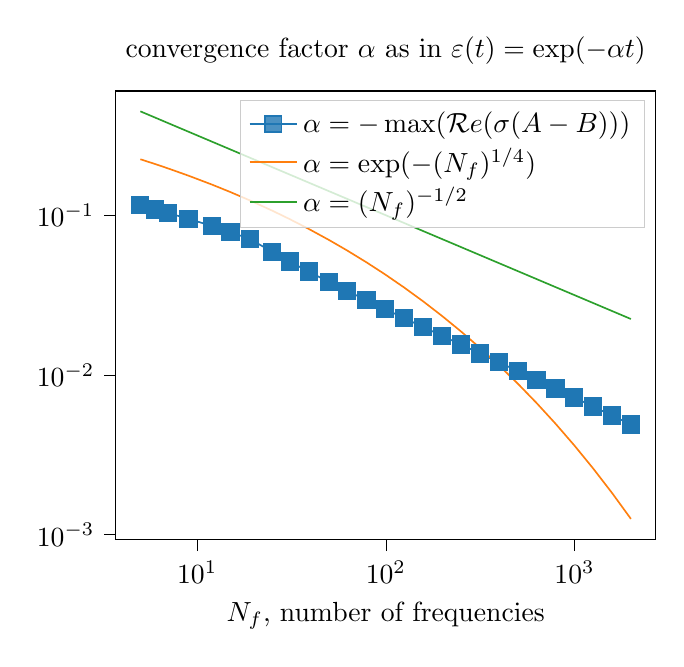
\begin{tikzpicture}

\definecolor{darkgray176}{RGB}{176,176,176}
\definecolor{darkorange25512714}{RGB}{255,127,14}
\definecolor{forestgreen4416044}{RGB}{44,160,44}
\definecolor{lightgray204}{RGB}{204,204,204}
\definecolor{steelblue31119180}{RGB}{31,119,180}

\begin{axis}[
legend cell align={left},
legend style={fill opacity=0.8, draw opacity=1, text opacity=1, draw=lightgray204},
log basis x={10},
log basis y={10},
tick align=outside,
tick pos=left,
title={convergence factor $\alpha$ as in $\varepsilon(t) = \exp(-\alpha t)$},
x grid style={darkgray176},
xlabel={$N_f$, number of frequencies},
xmin=3.70660110378415, xmax=2684.39999919113,
xminorgrids,
xmode=log,
xtick style={color=black},
xtick={0.1,1,10,100,1000,10000,100000},
xticklabels={
  $\mathdefault{10^{-1}}$,
  $\mathdefault{10^{0}}$,
  $\mathdefault{10^{1}}$,
  $\mathdefault{10^{2}}$,
  $\mathdefault{10^{3}}$,
  $\mathdefault{10^{4}}$,
  $\mathdefault{10^{5}}$
},
y grid style={darkgray176},
ymin=0.00093707847069596, ymax=0.599893283628659,
yminorgrids,
ymode=log,
ytick style={color=black},
ytick={1e-05,0.0001,0.001,0.01,0.1,1,10},
yticklabels={
  $\mathdefault{10^{-5}}$,
  $\mathdefault{10^{-4}}$,
  $\mathdefault{10^{-3}}$,
  $\mathdefault{10^{-2}}$,
  $\mathdefault{10^{-1}}$,
  $\mathdefault{10^{0}}$,
  $\mathdefault{10^{1}}$
}
]
\addplot [semithick, steelblue31119180, mark=square*, mark size=3, mark options={solid}]
table {%
5 0.115617907378508
6 0.108643850919702
7 0.103356458179086
9 0.09494835817188
12 0.0856283420351959
15 0.0785271301391885
19 0.0711014897373858
25 0.0590317228713167
31 0.0512704526445218
39 0.0444147245369646
50 0.0382508943046673
62 0.0337343140468278
79 0.0293699533546137
99 0.02586772181139
125 0.0227190783025284
158 0.0199601504402929
199 0.0175799373544776
250 0.015508711139742
315 0.013659570499955
398 0.0120112670542514
500 0.0105932614886845
629 0.00933378243440709
792 0.00821843697077153
997 0.00723568966790948
1255 0.00634930074272466
1581 0.00557528466457482
1990 0.00490290047454986
};
\addlegendentry{$\alpha = -\max(\mathcal{R}e(\sigma(A-B)))$}
\addplot [semithick, darkorange25512714]
table {%
5 0.22417040466647
6 0.20907032924167
7 0.196601476387258
9 0.176921206317764
12 0.155484424214303
15 0.139737492331243
19 0.123959840851917
25 0.106877925660386
31 0.0944569539732736
39 0.0821671740250601
50 0.0700078466319701
62 0.0604422894066576
79 0.0507264655662953
99 0.0426664600837311
125 0.0353060294075425
158 0.0288573055564157
199 0.0233795516560368
250 0.0187538982063671
315 0.014803880589163
398 0.0114870464651056
500 0.00883788181249389
629 0.00668438632552924
792 0.00496694654313548
997 0.00362757485175639
1255 0.00260070501189767
1581 0.00182587655930176
1990 0.00125699908602974
};
\addlegendentry{$\alpha = \exp(-(N_f)^{1/4})$}
\addplot [semithick, forestgreen4416044]
table {%
5 0.447213595499958
6 0.408248290463863
7 0.377964473009227
9 0.333333333333333
12 0.288675134594813
15 0.258198889747161
19 0.229415733870562
25 0.2
31 0.179605302026775
39 0.160128153805087
50 0.14142135623731
62 0.127000127000191
79 0.112508790092602
99 0.100503781525921
125 0.0894427190999916
158 0.079555728417573
199 0.0708881205008336
250 0.0632455532033676
315 0.0563436169819011
398 0.0501254707117086
500 0.0447213595499958
629 0.039872611141445
792 0.0355334527259351
997 0.0316703177609768
1255 0.0282278718468818
1581 0.0251497727413928
1990 0.022416791983111
};
\addlegendentry{$\alpha = (N_f)^{-1/2}$}
\end{axis}

\end{tikzpicture}
